%!TEX root = ../thesis.tex
%*******************************************************************************
%****************************** Second Chapter *********************************
%*******************************************************************************

\chapter{Related Work}

\ifpdf
    \graphicspath{{Chapter3/Figs/Raster/}{Chapter3/Figs/PDF/}{Chapter3/Figs/}}
\else
    \graphicspath{{Chapter3/Figs/Vector/}{Chapter3/Figs/}}
\fi

\section{Introduction}

This section will discuss a variety of related work.

\section{Methods for 2D/3D skeletal fitting}

The first class of techniques, known as \textit{skeletal fitting} methods, recover detailed pose attributes from the target but learn only weak shape attributes. As these methods only ever return a skeletal outline, apart from basic limb measurements, no other shape detail (e.g. surface definition, object density etc.) is obtained. However, it is important to note that this is often perfectly satisfactory, and wholly dependent on the intended use-case. In particular, such techniques have found numerous applications in controllerless gaming and for other human-computer interaction purposes. Early approaches worked by building statistical models of limb lengths and poses using freely available motion capture data~\cite{barron2001estimating}. These could then be used to adapt a digital skeleton to fit each frame of an input video sequence. 

\subsection{Kinect body joint prediction}
Shotton et al. \cite{kinectpaper} designed a notable approach in this category by designing a human skeletal tracking capability later incorporated into the Microsoft Kinect Sensor SDK (see Figure \ref{fig:kinect_skeleton}. A large motion capture database containing approximately 500K frames was captured from human subjects performing a wide variety of activities (e.g.\ driving, dancing, kicking, running, etc.). This dataset was then used to drive a generative body model (constituting strong prior knowledge for this problem) which could be sampled from to create synthetic depth images with dense body part labels. A random forest classifier is then used to predict these body labels on unseen examples. A per-pixel density estimator for each body part is calculated for each 3D world space coordinate based on: (1) the inferred body part probability for the projected pixel, (2) the world surface area of the pixel. Density estimators for each body part are then used in combination to localize particular body joints, which are annotated with a calculated confidence value. 

\begin{figure}[H] % Example image
    \center{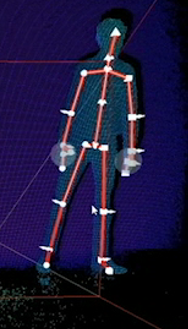
\includegraphics[width=0.25\linewidth]{human_tracking}}
    \caption{Kinect generating per-pixel joint proposals.}
    \label{fig:kinect_skeleton}
\end{figure}

\subsection{Multi-stage approaches}
More recent approaches are either predict 2D joint positions on an input image, and use a subsequent step that `lifts' these to a 3D pose, or predicts the 3D pose directly. Note that both approaches must overcome significant ambiguity. Determining joint positions is a task made challenging due to large variations in visual appearence, commonly due to clothing, body shape and camera view. As explained by Toshev and Szegedy~\cite{toshev2014deeppose}, even with perfect joint locations the subsequent lifting step is also ill-posed, as the space of consistent 3D poses for given 2D landmark locations is infinite. This is typically resolved using strong prior knowledge which usually takes the form of 3D geometric pose priors and temporal or structural constraints. Examples of such systems include DeepPose~\cite{toshev2014deeppose}, an approach which employs a CNN to reason jointly about 2D landmark detection and 3D pose estimation from single RGB images. Pishchulin et al.~\cite{pishchulin2016deepcut} later introduced DeepCut which extends DeepPose to the multi-person case. Both systems are trained on large body joint databases. 

\subsection{Direct approaches}
However, some direct techniques exist which do not require an initial 2D joint prediction. These include methods that directly regress to a 3D pose~\cite{tekin2016direct}. However, these typically rely on an annotated set of 3D joint labels, which can be difficult and costly to obtain, or being able to build a representative synthetic dataset, which is non-trivial task.

%% Discuss Amazon's system, Novotny's system etc.

\subsection{Discussion on applicability to animals}
% 2D predictor DeepLabCut 

\section{Model-free dense 3D reconstruction}

This section will discuss methods for dense 3D reconstruction. 

\begin{enumerate}
    \item PiFu and Neural Radiance Fields
    \item Novotny dense 3D prediction
\end{enumerate}

\section{Model-based dense 3D reconstruction}

We want to do model based reconstruction to impose a prior on the fitting and also automatically recover an interpretable fit. 

\subsection{Fitting to animal video sequences}
Stebbing et al.~\cite{arap_stebbing} introduce a technique capable of fitting a template mesh to live video sequences for a range of different animal species. Some user interaction is required in order to segment the animal from the background and to provide sparse 3D-mesh-to-2D-image key point correspondences. This work only operates on input video sequences (rather than single frames), so a number of temporal terms are incorporated that encourage sensible inter-frame model deviation. The system requires an annotated input template mesh representative of the target animal species. Note that this work does not require the template mesh to have an inner skeletal structure. However, the user assists an ARAP-style term by assigning each mesh vertex $v_i$ to one of $M$ groups which share a set of basis rotations $B_{m}$. 

\begin{figure}[H]
    \centering
    \begin{subfigure}{0.5\textwidth}
    \centering
        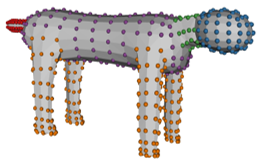
\includegraphics[height=0.5\linewidth]{arapsfm/arap_annotated_template}
        \caption{Template mesh with joint movement constraints.}
    \end{subfigure}%
    \begin{subfigure}{0.5\textwidth}
    \centering
        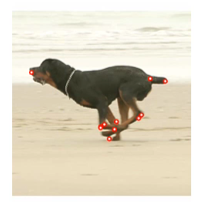
\includegraphics[height=0.5\linewidth]{arapsfm/arap_point_tracks}
        \caption{Example of user supplied point tracks.}
    \end{subfigure}%
    \caption{User input required for the deformable mesh animation algorithm, reprinted from~\cite{arap_stebbing}.}
    \label{fig:arap_user}
\end{figure} 

Through reasonably accurate pose fitting and by allowing some pose-invariant shape deformation, this work produces smooth meshes which are often a good match to the input video. Moreover, their experimentation shows that ARAP is a useful prior for reconstructing articulated, non-rigid motion in instances that an internal skeleton is a priori unknown. However, the shape attributes for the reconstructed model are not particularly accurate, which results in frequent errors appearing at internal occluding contours. In addition, the large non-convex optimization algorithm is an expensive operation, taking around 1 minute per video frame on a standard Linux workstation.

Results showing this work fitting a crude dog template mesh to a sample video obtained from YouTube are shown previously in Figure \ref{fig:intro_arap_output}. Figure \ref{fig:arap_output} shows another example, which operates on a template impala mesh.

\begin{figure}[H]
    \center{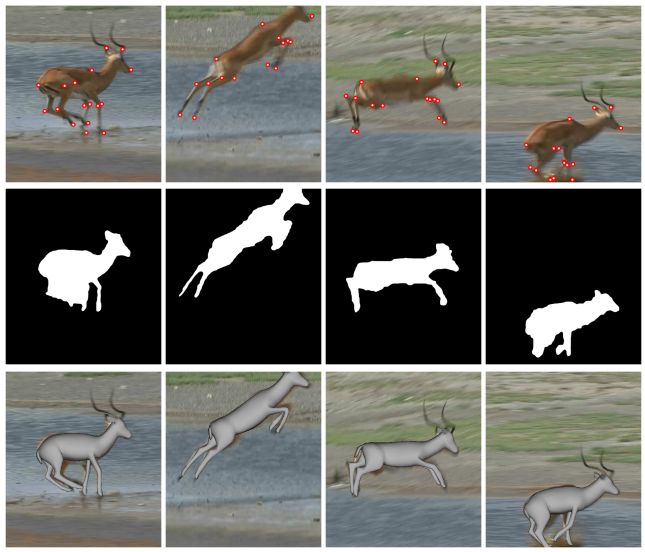
\includegraphics[width=0.95\linewidth]{arapsfm/arap_impala}}
    \caption{Example of an impala template being fit to input video sequence, reprinted from~\cite{arap_stebbing}}
    \label{fig:arap_output}
\end{figure}

\subsection{Learning animal shape from unrelated 2D images}
Cashman and Fitzgibbon~\cite{cashman2013shape} introduce an optimization technique able to recover a parameterized, morphable 3D model from unrelated 2D images depicting examples of the target class. The method requires user-supplied 2D object outlines and point constraints for each image, and a single rigid mesh for the entire object class. The authors demonstrate recovering an 8-parameter morphable dolphin model from 32 images obtained from Google. To reduce required user activity, it is reasonable to assume that given sufficient labelled training data, it would be simple to manipulate a convolutional network architecture able to perform foreground / background segmentation and identify human key points (say, joints) for the desired object class. The system achieves impressive results when optimizing over both pose and shape parameters across a range of object classes, but struggles for articulated models such as polar bears.

\begin{figure}[H] % Example image
    \center{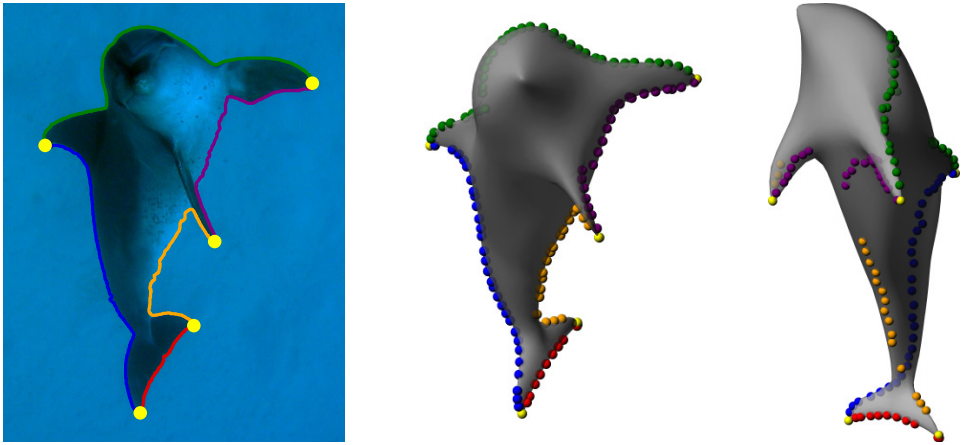
\includegraphics[width=0.7\linewidth]{dolphins}}
    \caption{8-parameter dolphin model with annotated contour (left) and contour generators (middle and right).}
    \label{fig:cashman_fitzgibbon}
\end{figure}

\subsection{Fitting to an articulated hand model}
Given the availability of strong shape and pose priors, articulated hand tracking aptly demonstrates the advantage of model fitting approaches. Again, it is first necessary to decide how the human hand should be parameterized, i.e. what an optimizer should specifically aim to learn. Similar to the case with the full human body, the aim is again to adapt a mesh (although this time of a hand) to reproduce a performance given by a real human hand either in still frames or from an input video sequence. Many modern approaches follow a hand parameterization given by Khamis et al.~\cite{Khamis_2015_CVPR} using a pose vector $\theta \in \mathbb{R}^{28}$ that includes global translation and rotation, one adbuction and three flexion variables for each finger digit, and one abduction and flexion parameter for the wrist and forearm. An example hand tracking result can be seen in Figure~\ref{fig:hand_tracking}. 

\begin{figure}[H] % Example image
    \center{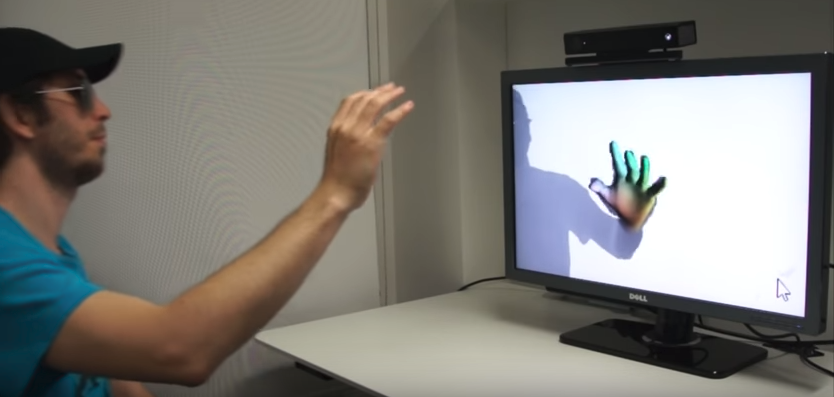
\includegraphics[width=0.85\linewidth]{hand_tracking}}
    \caption{Example of articulated hand tracking, reprinted from~\cite{taylor2016efficient}.}
    \label{fig:hand_tracking}
\end{figure}

\subsection{Data-driven body models}
Data-driven statistical body models built from large database of human 3D scans are receiving increasing attention from the research community. Having been trained on examples of real humans of a range of different shapes and adopting various poses, these models capture subtle details that is hard to encode explicitly. In part due to a good choice of training candidates, SCAPE~\cite{anguelov05scape}, FAUST~\cite{bogo2014faust} and SMPL~\cite{loper15smpl} models exemplify this technique and are able to account for many body shapes, poses and non-rigid deformations such as muscle bulging due to joint articulation. The quality of such models is such that a user can construct visually-realistic bodies that were never present in the original data. A noteable drawback of such approaches is the required time and financial investment in conducting the data capture and the subsequent need to align each scan.

SMPL first learns how human beings deform through pose changes using 1786 high-resolution 3D scans of different subjects in a wide variety of poses. Following alignment to a template mesh, a linear model for each biological gender is created from the CAESAR dataset \cite{robinette2002civilian} using principal component analysis (PCA). SMPL was motivated by the ambition to generate a realistic data-driven human body model which can be rendered in real-time using standard engines, such as Unity~\cite{unity2017} or Blender~\cite{blender2017}. Having been designed for animation, SMPLs base template has a number of useful qualities for this work; the underlying mesh is a clean structure and comprises relatively few polygons. A novelty of this model is that it encodes explicit and meaningful body joint positions. Some sample SMPL meshes are shown in Figure \ref{fig:smpl_model}.

\begin{figure}[H] % Example image
    \center{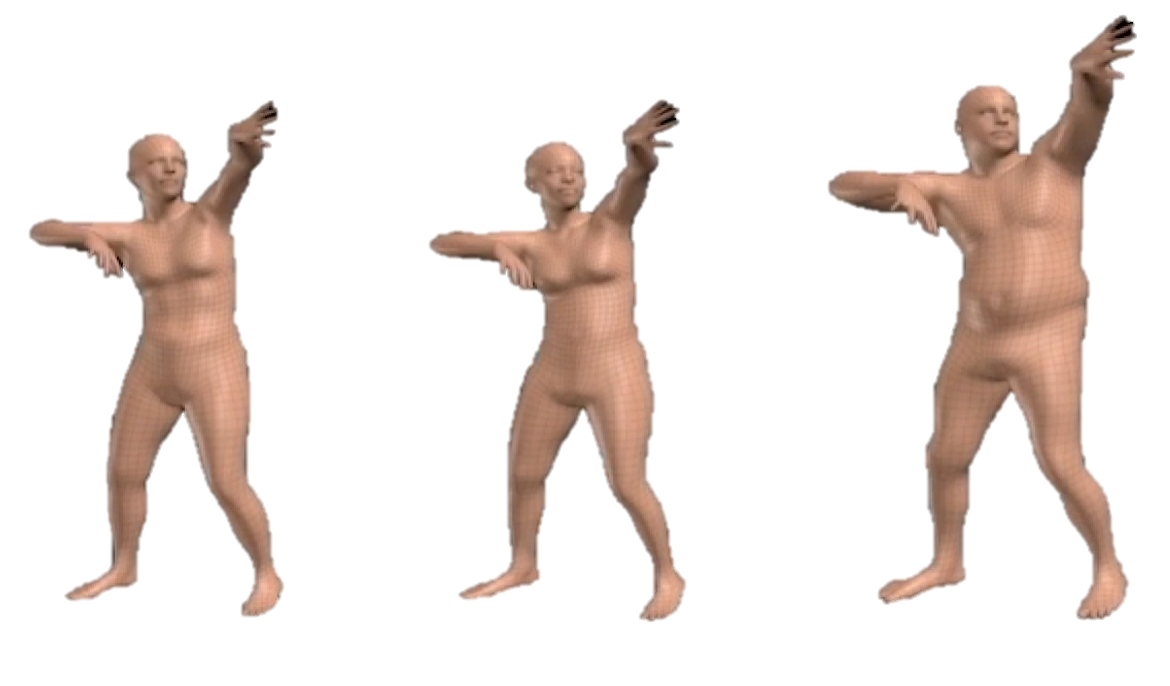
\includegraphics[width=0.5\linewidth]{smpl_wbg}}
    \caption{SMPL model showing pose-invariant shape changes, reprinted from~\cite{loper15smpl}.}
    \label{fig:smpl_model}
\end{figure}

A similar technique to that used to build the SMPL model has been recently used to build a Skinned Multi-Animal Linear Model (SMAL)~\cite{zuffi2017menagerie}, a generative animal model exhibiting realistic 3D shape (see Figure \ref{fig:smal_model_shape}) and pose (see Figure \ref{fig:smal_model_poses}). Due to the lack of available motion capture data for animal subjects, the SMAL model is learnt from a set of $41$ 3D scans of toy figurines in arbitrary poses. The figurines span five quadruped families, and included examples of lions, cats, tigers, dogs, horses, any many more, although notably for this work no rodent toys were included. The paper introduces a new technique to accurately align each toy scan to a common template, allowing the shape space to be learnt.

\begin{figure}[H]
    \centering
    \begin{subfigure}{0.3\linewidth}
    \centering
        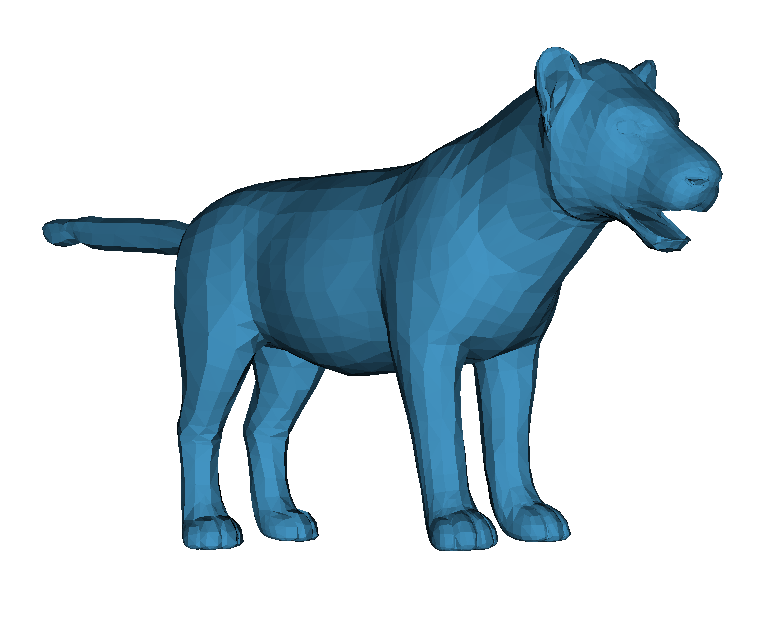
\includegraphics[width=1\linewidth]{smal/default}
        \caption{Default SMAL mesh.}
    \end{subfigure}%
    \begin{subfigure}{0.3\linewidth}
    \centering
        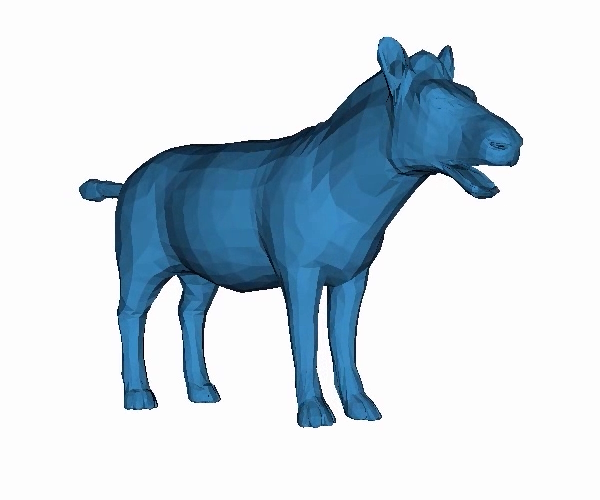
\includegraphics[width=1\linewidth]{smal/horse}
        \caption{SMAL in horse shape.}
    \end{subfigure}%
    \begin{subfigure}{0.3\linewidth}
        \centering
            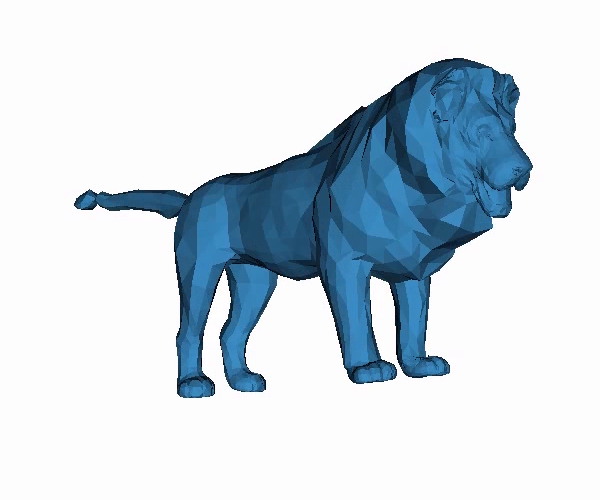
\includegraphics[width=1\linewidth]{smal/lion}
            \caption{SMAL in lion shape.}
    \end{subfigure}%
    \caption{SMAL with varying shape parameters.}
    \label{fig:smal_model_shape}
    \end{figure}

    \begin{figure}[H]
    \centering
    \begin{subfigure}{0.3\linewidth}
    \centering
        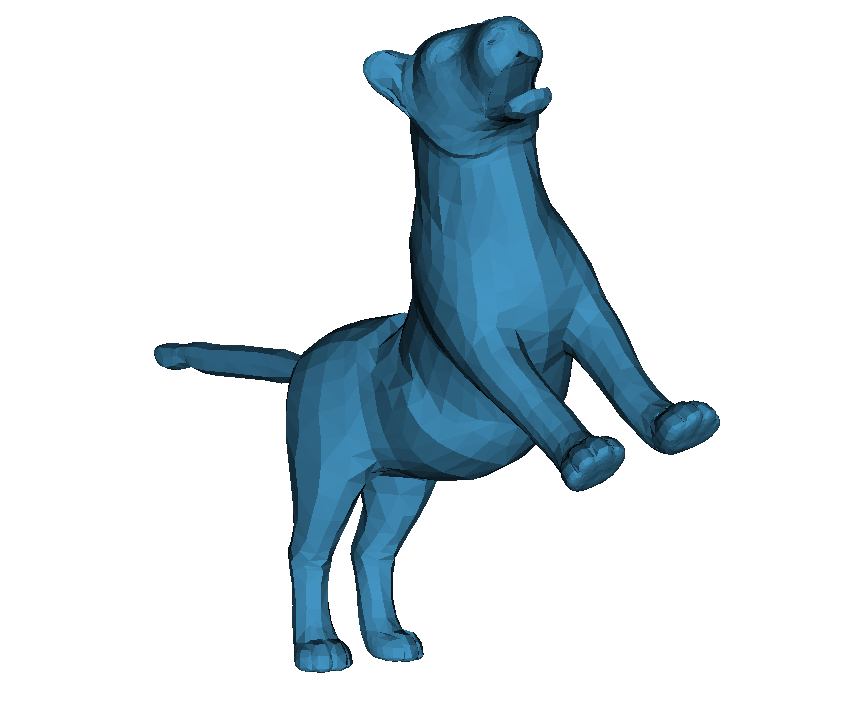
\includegraphics[width=1\linewidth]{smal/pose_1}
    \end{subfigure}%
    \begin{subfigure}{0.3\linewidth}
    \centering
        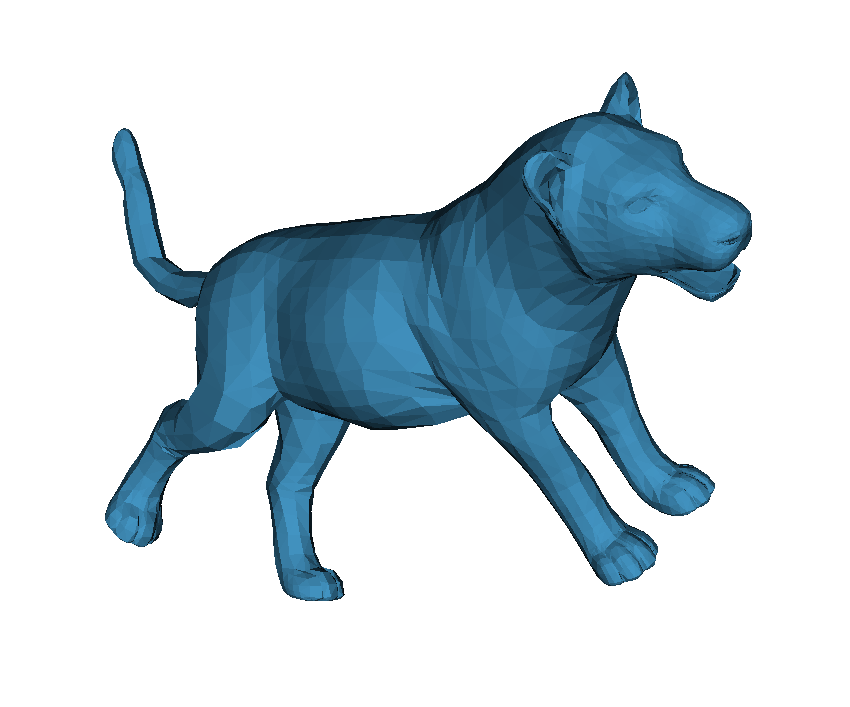
\includegraphics[width=1\linewidth]{smal/pose_2}
    \end{subfigure}%
    \begin{subfigure}{0.3\linewidth}
        \centering
            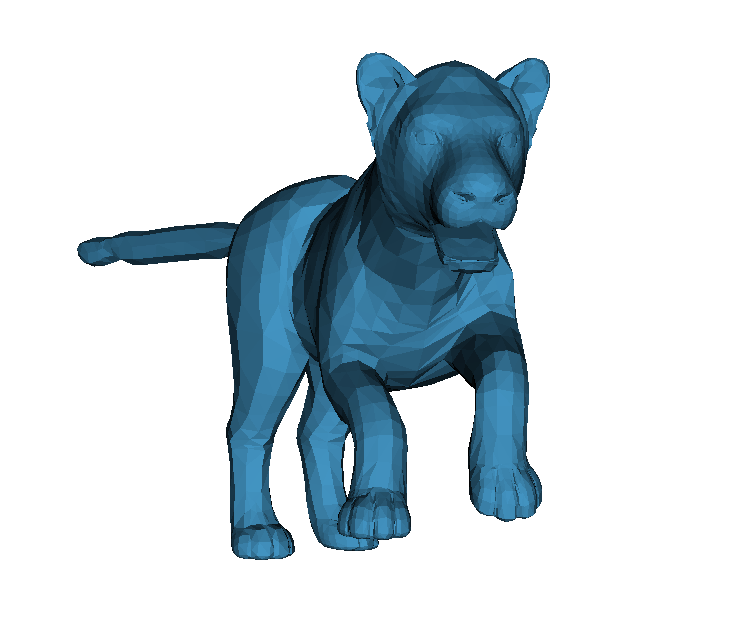
\includegraphics[width=1\linewidth]{smal/pose_3}
    \end{subfigure}%
    \caption{SMAL with varying pose parameters.}
    \label{fig:smal_model_poses}
\end{figure}

From the paper, SMAL is defined as a function $M(\beta, \theta, \gamma)$ parameterized by pose-invariant shape $\beta$, pose $\theta$ (including global rotation) and global translation $\gamma$. The function returns a triangulated surface comprising $6890$ vertices. SMAL contains $41$ shape parameters $\beta$ which are coefficients of a low-dimensional shape space. There are three pose parameters for each of the $32$ body joints and an additional three to express the global rotation. Global translation $\gamma$ is expressed by a further three parameters.

\subsubsection{Fitting the SMPL mesh to human images}
SMPLify \cite{bogo16keep} is a fully-automated optimization approach that uses predicted human joint positions to constrain a optimizer that fits the aforementioned SMPL model to RGB input images. It first makes use of the DeepCut CNN to predict 2D human body joints $J_{\text{est}}$ on input frames. For each 2D joint $i$ the CNN is able to provide a confidence value $w_i$ for the joint's position. The optimization begins by first solving for global rotation (i.e. $\theta_{0..2}$) and global translation $\gamma$ by fitting a small number of 2D torso points $J_{\text{torso}} \subset J_{\text{est}}$ to the data. The user is expected to provide a value for the focal length $f$. Then, the full optimization takes place, fitting 3D pose and shape to all 2D joints by minimizing the following objective function which comprises five error terms:

\begin{equation}
E(\beta, \theta) = E_{J}(\beta, \theta; K, J_{\text{est}}) + \lambda_{\theta}E_{\theta}(\theta) + \lambda_{\alpha}E_{\alpha}(\theta) + \lambda_{\text{sp}}E_{\text{sp}}(\theta; \beta) + \lambda_{\beta}E_{\beta}(\beta)
\end{equation}
where $\lambda$ terms are the scalar weights. The term $E_{J}$ is often referred to as the \textit{data} term, as it places most emphasis on constraining the model to the input sensory data. The job of this term is to penalize the weighted 2D distance between estimated joints $J_{\text{est}}$ and corresponding projected SMPL joints. In practice, this projection takes place using the OpenDR differentiable rendering framework to ensure the final formulation remains differentiable:

\begin{equation}
    E_{J}(\beta, \theta; K, J_{\text{est}}) = \sum_{joint j} w_{j} \rho(\Pi_{K}(R_{\theta}(J(\beta)_j)) - J_{\text{est}, j})
\end{equation}
where $J(\beta)$ is a function which predicts 3D body joints from body shape and $R_{\theta}(J(\beta))$ therefore denote posed 3D joints.

The remaining terms are now briefly discussed:
\clearpage
\begin{itemize}
    \item $E_{\theta}(\theta)$ is referred to as a \textit{pose prior} which favours more likely poses by assigning large punishment to those that deviate from known poses collected from a large dataset.
    \item $E_{\beta}(\beta)$ is referred to as a \textit{shape prior} which favours more likely pose-invariant shape configurations by assigning large punishment to those that deviate from known shapes collected from a large dataset. 
    \item $E_{\alpha}(\theta)$ is a \textit{joint limit} prior which ensures particular joints remain within acceptable angle limits. For example, a knee joint in a human model should be prohibited from bending more than 5 degrees upwards.
    \item $E_{sp}(\theta; \beta)$ is an \textit{interpenetration} term, which can only be defined in such shape modelling approaches. Using both shape and pose from the model, it is possible to determine if any limbs are self-intersecting, or intersect other parts of the body and assign appropriate penalty.
\end{itemize}

An example result can be seen in Figure \ref{fig:smplify}:

\begin{figure}[H] % Example image
    \center{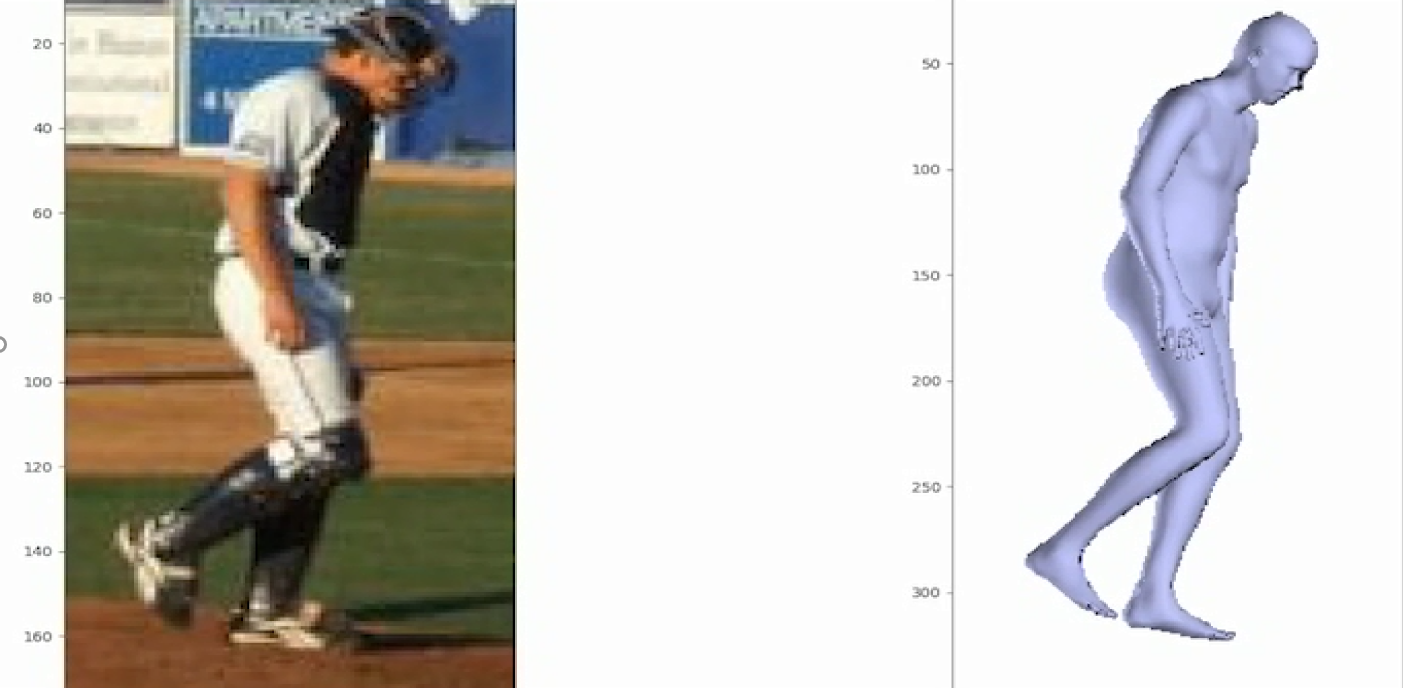
\includegraphics[width=0.95\linewidth]{fitting_smpl}}
    \caption{SMPLify: Fitting the SMPL model to the Leeds Sports Dataset.}
    \label{fig:smplify}
\end{figure}

\subsubsection{Fitting the SMAL mesh to animal images}
The SMAL paper briefly discusses a modification to the SMPLify approach in order to fit the SMAL model to RGB animal input images. The terms are largely the same, although the interpenetration term is omitted and joint positions are provided manually, rather than being predicted by a CNN. Finally, the optimizer requires a pre-segmented (i.e.\ silhouette) image which is also supplied by a user. An approach discussed in Chapter 4 builds on this work, so an in-depth description of this method is ommited here. However, an example result showing the result of the optimizer fitting the SMAL mesh to an RGB image of a fox can be seen in Figure \ref{fig:smalify}. Note that the whole optimization process takes around 1 minute per frame.

\begin{figure}[H] % Example image
    \center{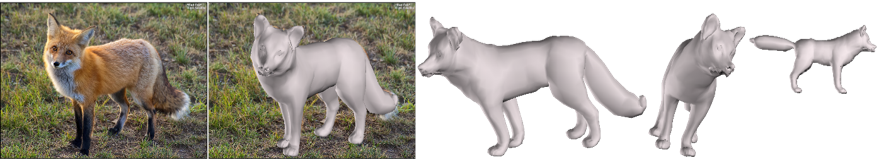
\includegraphics[width=0.95\linewidth]{fitting_smal}}
    \caption{Fitting SMAL to a hand segmented animal, reprinted from~\cite{zuffi2017menagerie}.}
    \label{fig:smalify}
\end{figure}

        
\subsection{Direct regression}
The most recent, and state-of-the-art approaches employ deep learning techniques to solve the entire optimization problem by directly regressing to shape and pose parameters of the template model. Tekin et al.~\cite{tekin2016direct} introduce a convolutional network trained on the Human3.6m dataset~\cite{lin2014microsoft} that directly regresses to a human pose defined in terms 3D locations $y \in \mathbb{R}^{3J}$ of $J$ body joints relative to a root joint. Tan et al.~\cite{tan17indirect} introduce an approach that directly regresses to SMPL parameters from synthetic images, ensuring suitable image jitters are applied to promote generality to real-world images. The method is termed Indirect Learning, and is trained from real human images with no known corresponding SMPL parameters. An autoencoder network is introduced, and a decoder first trained from synthetic (SMPL parameter, rendered image) pairs to construct an automatic renderer. This part of the network is then frozen, before the entire autoencoder is trained on many segmented human images that optimize the encoder to real-world examples. The end result is a process that is able to predict SMPL parameters from real-world human images. An example result is shown in Figure~\ref{fig:indirect_learning}.

\begin{figure}[H] % Example image
    \center{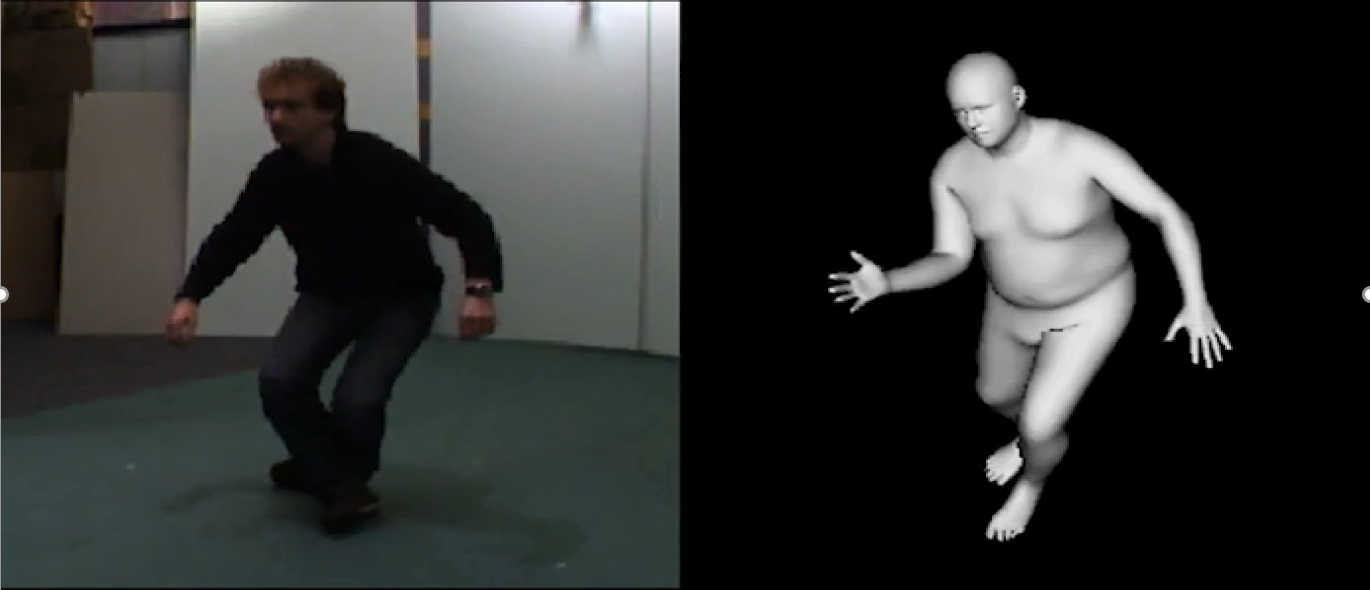
\includegraphics[width=0.75\linewidth]{indirect_learning}}
    \caption{Indirect learning method regressing to SMPL parameters from an RGB video sequence. Reprinted from~\cite{tan17indirect}.}
    \label{fig:indirect_learning}
\end{figure}


    
% \section{Obtaining animal test data}
%     A significant drawback due to the lack of available training data is that state-of-the-art segmentation pipelines require a wealth of (RGB Input, Segmentation) and (IR Input, Segmentation training pairs which are not readily available for animal targets. To resolve this, a collaborative project is underway between GSK and Texuna to design a bespoke camera module which can be fit into rodent, dog, mini-pig and rabbit enclosures. Figure \ref{fig:texuna_cage} shows a recent prototype design. The cameras are able to flip between RGB and IR capture modes and use IP camera technology, which is supported by a number of off-the-shelf recording systems. Once animal data is successfully recorded, it will be passed to human annotators to create a suitable dataset to train a segmentation network. Until this has been obtained, the system is designed on the premise of receiving perfect silhouette segmentations. 

%     % Talk a little more about the data -- problems (all outside?), occlusions, pets, number of pictures per animal (distribution) 
%     For testing, there are examples of real-world animal segmentations that form a satisfactory set for system testing. Between the Weizmann Horse Dataset~\cite{weizmann}, the IIIT-OXFORD PET dataset~\cite{oxfordpetdata} and animal superclasses from popular datasets such as MS Coco~\cite{lin2014microsoft} and PASCAL VOC~\cite{everingham2010pascal}, there are approximately one thousand RGB-segmentation pairs for independent images (i.e.\ not part of an available video sequence). It is worth noting that the distribution of images is heavily weighted towards cats, dogs and horses over other animal species. Moreover, images tend to be taken in outdoor environments with side-on animal views. This bias has been partially resolved by sourcing an additional 1500 frames from YouTube and the BBC Blue Planet II documentary series\footnote{Appropriate permissions have been sought where applicable}. These sequences were all segmented by hand, using the RotoBrush tool provided by the Adobe After-Effects~\cite{Bai:2009:VSC} package.  


\newcommand{\awfhang}[1]{
\begin{minipage}[t]{\textwidth}% Top-hanging minipage, will align on
                               % bottom of first line
\begin{tabbing} % tabbing so that minipage shrinks to fit
\\[-\baselineskip] % Make first line zero-height
#1 % Include user's text
\end{tabbing}
\end{minipage}} % can't allow } onto next line, as {WIDEBOX}~x will not tie.

\newcolumntype{L}[1]{>{\RaggedRight\hspace{0pt}}p{#1}}
\newcolumntype{R}[1]{>{\RaggedLeft\hspace{0pt}}p{#1}}

\begin{table}[t!]
{\sffamily
\scriptsize
\def\hd#1{\awfhang{#1}}
\begin{tabular}{@{}L{20mm}%Paper
|L{12mm}%Class
L{15mm}%Train
|L{15mm}%Template
L{17mm}%Video
L{17mm}%Test
|L{9mm}%Model
L{5mm}%Size
@{}}
\hd{Paper}%
&\hd{Animal\\Class}%
&\hd{Training\\requirements}%
&\hd{Template\\Model}%
&\hd{Video\\required}%
&\hd{Test Time\\Annotation}%
&\hd{Model\\Fitting}%
&\hd{Test\\Size}%
\\\hline
%%%%%%%%%%%%%%%%%%%%%%
This paper
& Dogs  % 2D Joints, Silhouettes, 3D Template, 3D Priors
& J2, S2, T3, P3
& SMAL
& No & None & No & 1703
\\\hline
%%%%%%%%%%%%%%%%%%%%%%
3D-Safari~\cite{Zuffi19Safari}        
& Zebras, horses
% 3D models (albeit synthetic), 2D Joints,  Silhouettes,  3D Priors
& M3 (albeit synthetic), J2, S2, P3
& SMAL
& 3-7 frames / animal & None & Yes & 200
\\\hline
%%%%%%%%%%%%%%%%%%%%%%
Lions, Tigers and Bears (SMALR)~\cite{zuffi_lions} 
& MLQ
& Not trained
& SMAL
& 3-7 frames / animal & J2, S2 & Yes & 14
\\\hline
%%%%%%%%%%%%%%%%%%%%%%
3D Menagerie (SMAL)~\cite{zuffi2017menagerie}                
& MLQ 
& Not trained
& SMAL
& No & J2, S2 & Yes & 48 
\\\hline
%%%%%%%%%%%%%%%%%%%%%%
Creatures Great and SMAL~\cite{biggs2018creatures}
& MLQ
& Not trained
& SMAL
& Yes & S2 (for best results shown) & Yes & 9             \\\hline 
%%%%%%%%%%%%%%%%%%%%%%
Category Specific Mesh Reconstructions~\cite{kanazawa2018birds}
& Birds
& J2, S2
& Bird convex hull
& No & None & No & 2850          
\\\hline
%%%%%%%%%%%%%%%%%%%%%%
What Shape are Dolphins~\cite{cashman2013shape}
& Dolphins, Pigeons 
& Not trained
& Dolphin Template
& 25 frames / category & J2, S2 & Yes & 25
\\\hline
%%%%%%%%%%%%%%%%%%%%%%
Animated 3D Creatures~\cite{reinert2016animatedsketching}
& MLQ
& Not trained
& Generalized Cylinders
& Yes & J2, S2 & Yes & 15
\\\hline
\end{tabular}
}
\caption{Literature summary: Our paper extends large-scale ``in-the-wild'' reconstruction to the difficult class of diverse breeds of dogs. 
MLQ: Medium-to-large quadrupeds. J2: 2D Joints. S2: 2D Silhouettes. T3: 3D Template. P3: 3D Priors. M3: 3D Model.}
\label{tab:literature}
% \vspace{-8mm}
\end{table}



